\section{Framework}
Through the discussed theory I have formulated a framework (see figure \ref{framework}) which takes influence from the Frogger Framework \cite{frogger} and is adapted it into a game design or game analysis context. The notions of augmented, inherent and functional information is transferred as they were aswell as the six aspects of time, location, direction, dynamics, modality and expression. A few aesthetic distinctions has been made to the visual representation of the framework to improve readability and functionality, as an example the horizontal division represents the division between feedforward on top and feedback at the bottom. This is done to avoid confusion that may arise when trying to discern if a coupling is through feedforward or feedback, which has arisen in other adaptations of the Frogger Framework \cite{tangifrog}. What follows here, however, addresses the changes made to the framework itself and not the aesthetic changes of a model.

\begin{figure}
  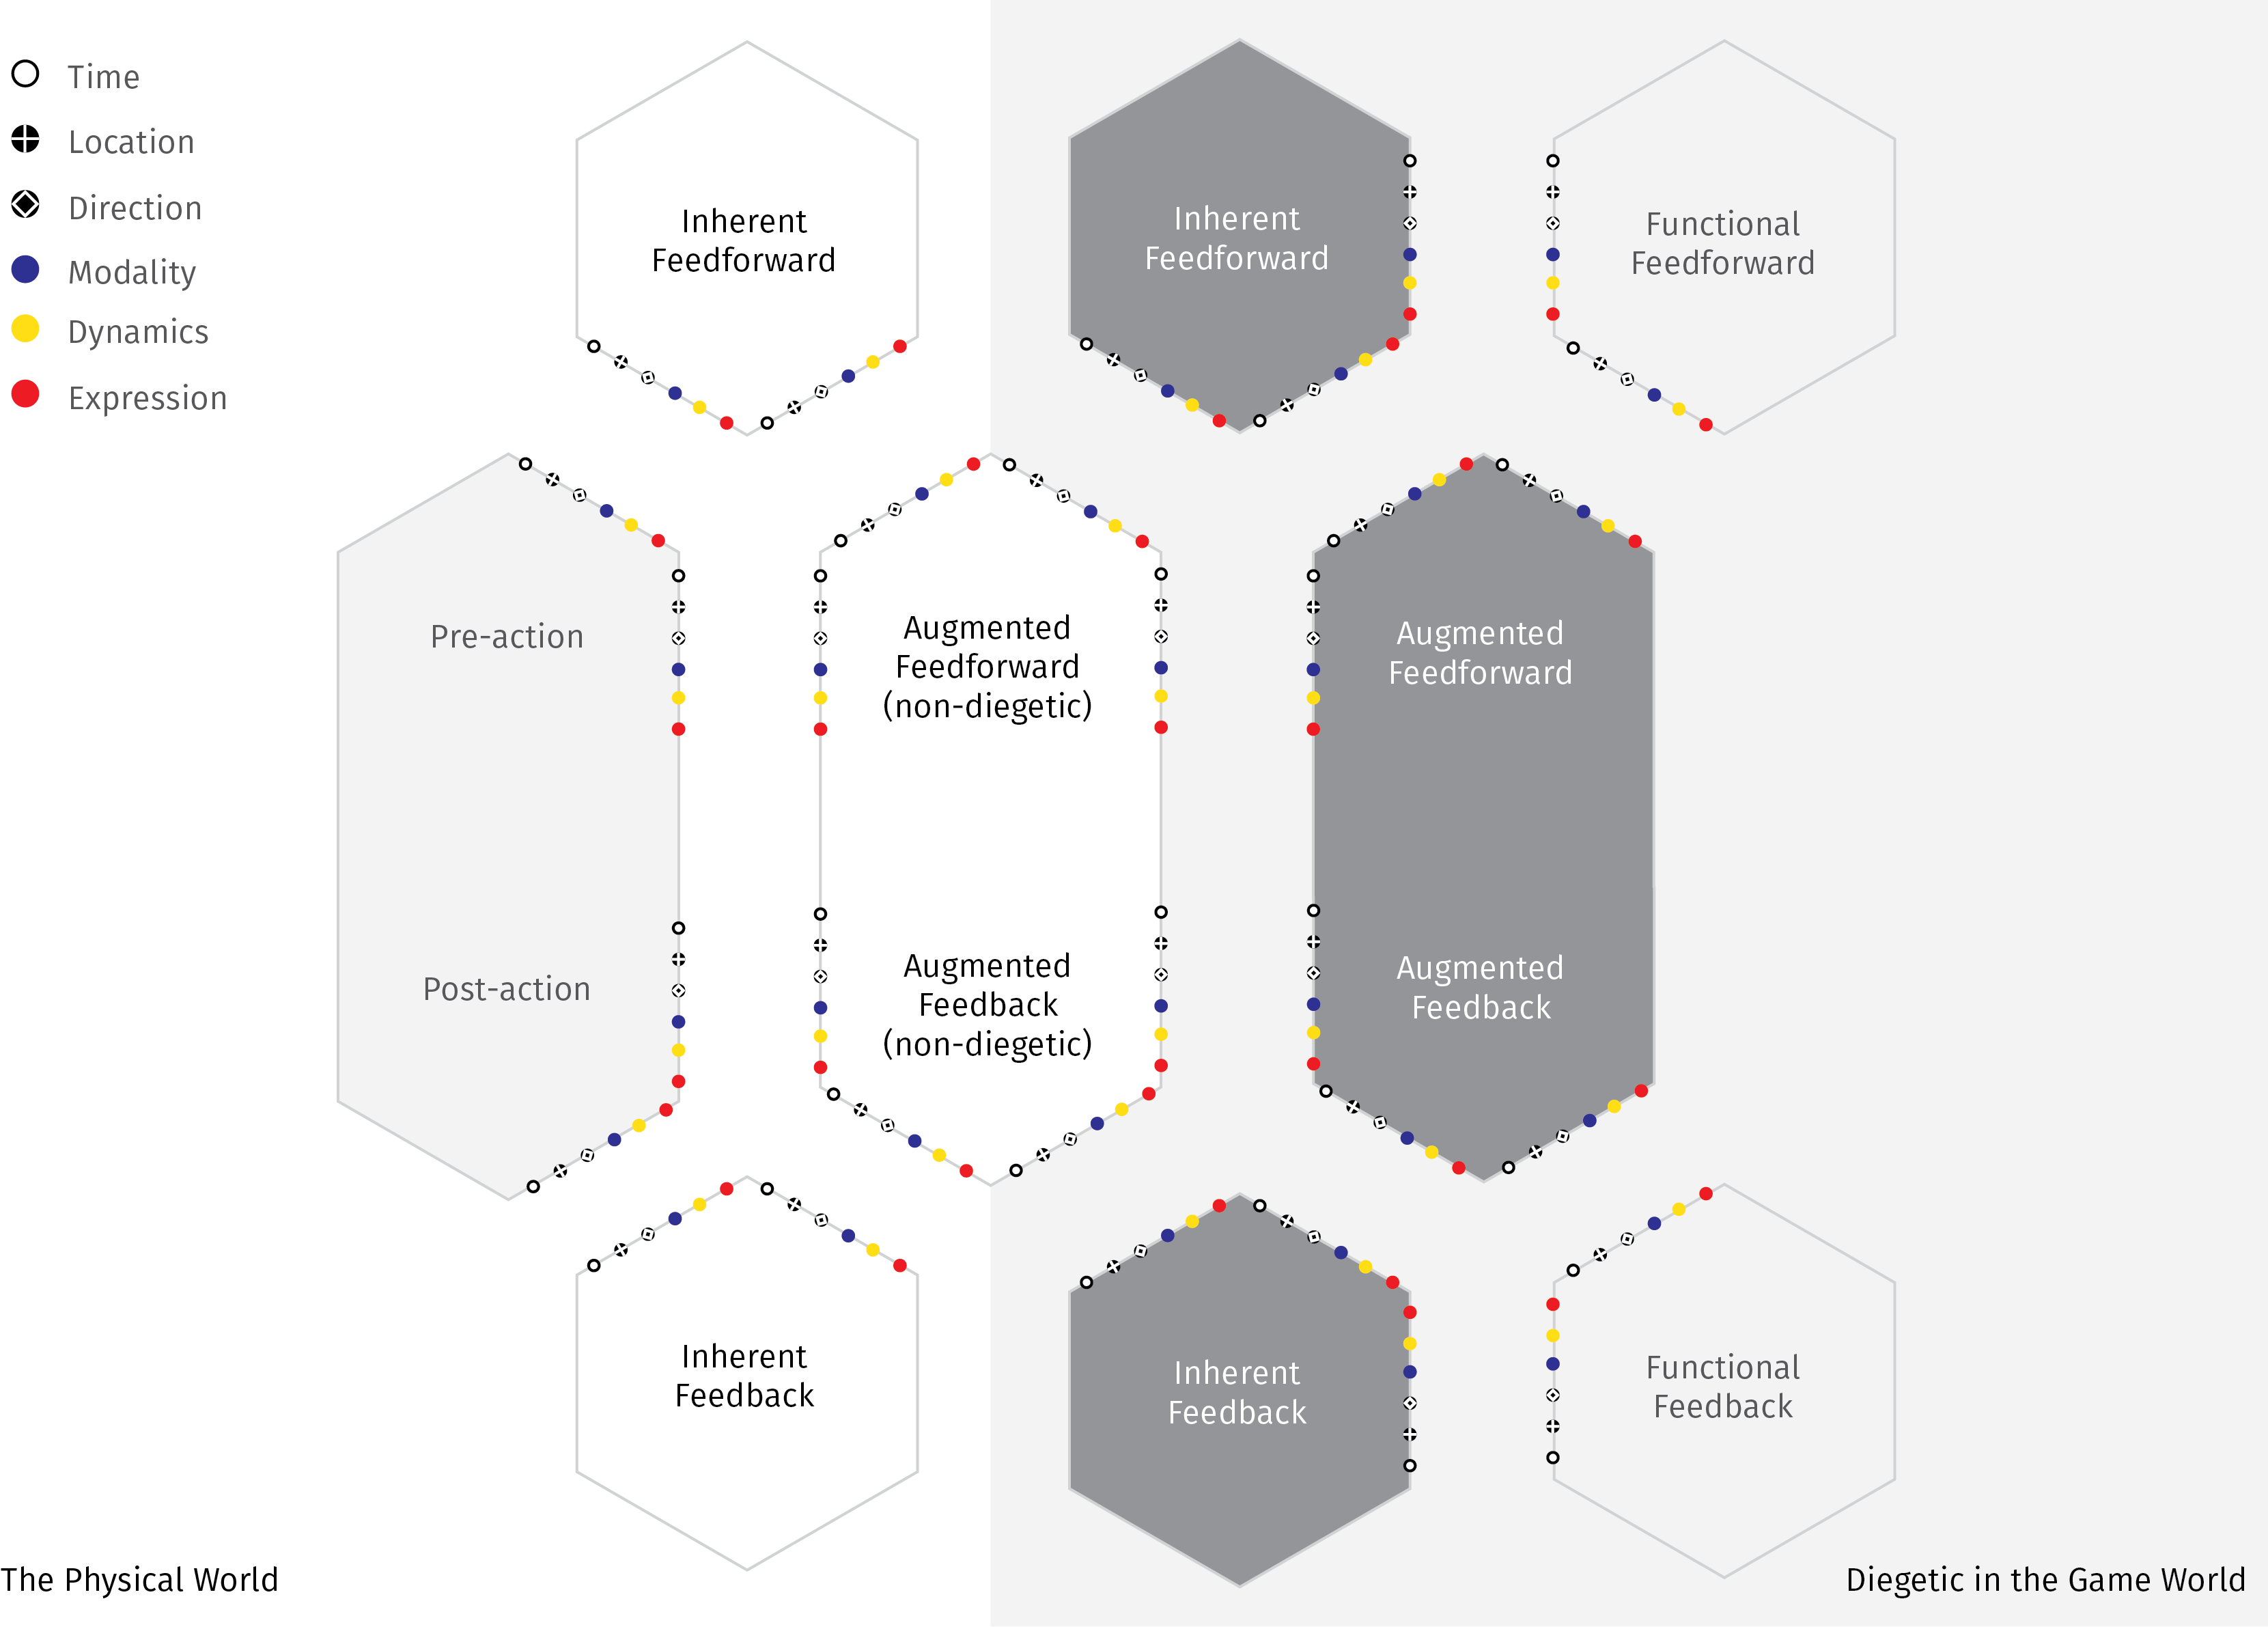
\includegraphics[width=\textwidth]{Framework}
  \caption{The Framework}
  \label{framework}
\end{figure}

\subsection{The Ludic Heterocosm}
The framework is divided on two axes. The horizontal, as discussed above, separates feedback from feedforward. The vertical division represents the division between the physical world and the game world. All things only existing in the physical world operates on the left side, and everything diegetic to the game world, i.e. what can be seen, heard, felt, tasted, smelled, touched, etc. by an entity in the game world operates on the game world side \cite{bordwell}. \citeA{vella} describes this world as the \textit{ludic heterocosm}. What is important to note about the ludic heterocosm is that it extends beyond what is visible on the screen at any one moment. It is an imagined world created in the player's mind. As an example, when meeting a travelling salesman of the Khajiit race in \citeA{skyrim}, the player may include the salesman's homeland of Elsweyr into her ludic heterocosm even though it is never visited in the game.

Even though both the game world and the physical world can be said to operate within Husserl's lebenswelt, the distinction has been made to address the detail that exists on both sides of the screen mediating a video game. On the physical side it can be the button layout of a Game Boy and on the game side it can be the shape of the incoming tetromino moving from top to bottom \cite{tetris}. With inherent and augmented information in the physical world being identical to the formulation in the Frogger Framework, what then becomes relevant to discuss is how augmented and inherent information is experienced in the ludic heterocosm.

The Frogger Framework definition uses concrete delimited designs like scissors and DVD-players \cite{frogger}, but has also been used to improve experiences like the Augmented Speed-skate Experience \cite{transbehav}. This is indicative of how the entire interaction experience is included in the framework, which is also imperative in a game context. Augmented information CAN BE FROM ANYWHERE.

Portal panels next to laser entries.

Game world Totten, Rollings, Vella

Inherent information is inherent from the action of the playable figure. Maybe Zelda Skyward Sword or Getting over it.

\subsection{Applying the Framework}
It is of great consideration when I make the distinction on the aspect of diegesis. A head-up display (HUD) is, as an example, usually not diegetic to the game world and therefore not existing for any agent within the game world. It can thus be said to provide meaning for the actions of the player and not the ludic subject, and therefore a HUD would usually be influential in regards to the augmented information of the physical world. What the framework's distinction then is attempting to mirror is the notion of involvement \citeA{calleja}. It can, however, not be said to integrate all six dimensions of involvement. The dimensions relevant to this framework is spatial involvement and kinaesthetic involvement. Spatial involvement is relevant because of the spatial point that is inhabited in the game world, and from this point the framework's aspects of location and direction relates. Kinaesthetic involvement is relevant because it is integral to a sense of control for the player and the fact that a close coupling on the six aspects of this framework leads to intuitive interaction \cite{frogger} should also lead to a higher degree of internalisation on the dimension of kinaesthetic involvement since it requires less attention as is also argued by \cite{calleja}:
\begin{quote}
  In the kinesthetic involvement dimension, conscious attention is generally dedicated to learning the controls of the game during a player’s early sessions of playing. This includes following on-screen instructions relating to avatar control or looking up and reassigning keys and buttons to the desired controls and then testing how these feel in the game. As players find the control setup that feels most intuitive to them or get used to the one supplied by the game, their conscious attention moves away from the basic controls to other aspects of the game. [...] In such cases, we can say that the player has 'internalized' the controls: she has reached a level of kinesthetic involvement that requires little or no conscious effort \cite[p. 45]{calleja}.
\end{quote}
Keeping in mind that any practical use of the framework in regards to design has the goal of improving intuitiveness of interaction, this means that the optimal use cases of the framework is when the player has not internalised the controls, since an internalisation would mean that the controls have indeed already become intuitive. Because of this, a relevant use case would be when a game introduces a \textit{game mechanic}, since the player would not have internalised the controls of the new mechanic at the time of the introduction, given that it is the first time playing.

Game mechanics can be defined in various ways, but for the context of this framework, the one offered by \citeA{sicartmechanic} is fitting: ``Game mechanics are methods invoked by agents, designed for interaction with the game state'' \cite{sicartmechanic}. \citeA{sicartmechanic} is borrowing from the terminology used in the field of object-oriented programming when he uses the word 'methods', but to clarify, he argues that these methods can be considered as verbs describing the action that is possible to be utilised by an agent. As an example, the player is able to ride a horse in \citeA{witcher}, which when considering methods as verbs makes 'riding' a game mechanic. In \citeA{witcher}, however, riding could be said to be comprised of several mechanics such as 'speeding', 'slowing' and 'halting'. \citeA{sicartmechanic} categorises these inclusive game mechanics as \textit{compound game mechanics}. In regards to granularity and the framework, the higher the detail, the less the confusion. If a compound game mechanic were to be described in the framework, the complexity created by the different sub-mechanics would in many cases lead to contradiction on the six aspects and the three types of information. A concern that is also addressed by \citeA{dourish} in regards to the complexity of computer systems:
\begin{quote}
  The consequence, then, is that there are very many different levels of description that could be used to describe my activity at any given moment. Some, perhaps, are ready-to-hand and some present-at-hand at the same time; my orientation toward them each will change. For instance, sometimes as I move the mouse, the mouse itself is the focus of my attention; some-times I am directed instead toward the cursor that it controls on the screen; at other times, I am directed toward the button I want to push, the e-mail message I want to send, or the lunch engagement I am trying to make \cite[p. 140]{dourish}
\end{quote}
Therefore, when designing or analysing the horse interaction in \citeA{witcher}, the mechanic to logically be addressed first is not 'riding' but 'mounting'. \\
Then, as discussed earlier, the framework should be used in the situation of introducing a player to a new game mechanic. This means that for the framework to be used, there needs to exist a game mechanic. It is therefore, not especially relevant in the initial formulation of a game mechanic. Where it does become relevant, is in the iteration thereafter. Examples of how this can be done follows later.

INTERACTION WITH THE GAME WORLD.


\subsection{Examples}
Game examples Witcher 3 horse riding

Zelda Skyward Sword and the enemies showing how to strike (direction).

Warioware

Something about symbolic, mimetic and symbiotic control being clearly visible on the physical world part of the model \cite[p. 64]{calleja}
